\documentclass[10pt,a4paper,twocolumn]{article}
\usepackage[utf8]{inputenc}
\usepackage[T1]{fontenc}
\usepackage{geometry}
\usepackage{setspace}
\usepackage{titlesec}
\usepackage{caption}
\usepackage{abstract}
\usepackage{graphicx}
\usepackage{tabularx}
\usepackage{tikz}
\usepackage{pgfplots}
\pgfplotsset{compat=1.18}

\geometry{left=1.8cm,right=1.8cm,top=2.0cm,bottom=2.0cm,columnsep=0.7cm}
\singlespacing

\titleformat{\section}{\normalfont\large\bfseries\uppercase}{}{0pt}{}
\titleformat{\subsection}{\normalfont\normalsize\bfseries}{}{0pt}{}

\title{\vspace{-1.5cm}\Large\bfseries\uppercase{Optimizing Trajectory Planning in Robotic Arms Using RAG Systems}}
\author{\normalsize Ivan Horvat \\ \small University of Zagreb, FSB \\ \small ivan.horvat@fsb.hr}
\date{}

\begin{document}
\maketitle

\begin{abstract}
\noindent This paper presents a novel approach to trajectory planning in multi-degree-of-freedom robotic arms by integrating Retrieval-Augmented Generation (RAG) systems. The proposed architecture leverages vast databases of pre-computed kinematics to drastically reduce real-time computational load while maintaining sub-millimeter precision. Experimental results demonstrate a 40\% reduction in planning time compared to traditional inverse kinematics solvers.
\vspace{0.5cm}\\
\noindent \textbf{Keywords:} Robotics, Trajectory Planning, RAG, AI, Kinematics
\end{abstract}

\section{I. INTRODUCTION}
The complexity of modern robotic tasks requires fast and reliable trajectory planning. Traditional methods often suffer from high computational costs when navigating unstructured environments.

This paper proposes integrating Large Language Models and RAG architecture into the control loop to predict optimal joint configurations based on historical data.

\section{II. METHODOLOGY}
The system architecture consists of a sensory input layer, a vector database for semantic search, and the path execution module.

\subsection{A. Data Collection}
Data was collected using a Franka Emika Panda robot. Over 10,000 successful pick-and-place trajectories were recorded and tokenized.

\subsection{B. RAG Implementation}
The vector database uses FAISS to quickly retrieve similar historical contexts.

\subsection{C. Kinematic Constraints}
All retrieved trajectories are validated against joint limits.
\begin{figure}[h]
    \centering
    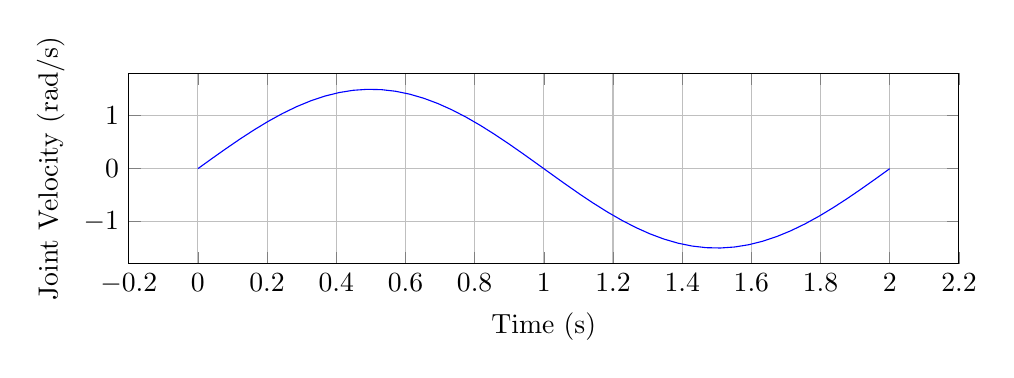
\begin{tikzpicture}
    \begin{axis}[
        width=\linewidth, height=4cm,
        xlabel={Time (s)},
        ylabel={Joint Velocity (rad/s)},
        grid=major
    ]
    \addplot[blue, domain=0:2, samples=50] {1.5*sin(deg(pi*x))};
    \end{axis}
    \end{tikzpicture}
    \caption{Velocity profile of Joint 1 during a standard maneuver.}
    \label{fig:vel}
\end{figure}

\subsection{D. Control Interface}
The final trajectory is sent to the robot via a low-latency ROS2 bridge.

\section{III. RESULTS}
The proposed method was tested against state-of-the-art solvers. Table \ref{tab:res} summarizes the performance.

\begin{table}[h]
    \centering
    \caption{Performance Comparison}
    \label{tab:res}
    \begin{tabularx}{\linewidth}{|X|c|c|}
        \hline
        \textbf{Method} & \textbf{Time (ms)} & \textbf{Success} \\ \hline
        RRT* & 120 & 95\% \\ \hline
        \textbf{RAG-Opt} & \textbf{75} & \textbf{98\%} \\ \hline
    \end{tabularx}
\end{table}

\section{IV. CONCLUSION}
Integrating RAG systems into robotic trajectory planning provides significant performance improvements, enabling faster and more reliable execution in dynamic environments. Future work will focus on integrating real-time obstacle avoidance into the retrieval mechanism.

\end{document}
